\subsection{Постановка задачи}
4.2. Реализовать метод стрельбы и конечно-разностный метод решения краевой задачи для ОДУ в виде программ. С использованием разработанного программного обеспечения решить краевую задачу для обыкновенного дифференциального уравнения 2-го порядка на указанном отрезке. Оценить погрешность численного решения с использованием метода Рунге – Ромберга и путем сравнения с точным решением. 

{\bfseries Вариант:} 20 (Сделан 21, поскольку 20 вариант прописан с ошибкой в файле с ТЗ)
    \begin{equation}
        x(2x+1)y'' + 2(x+1)y' - 2y = 0,\\
		y'(1)=0,\\
		y(3)-y'(3)=\frac{31}{9}
    \end{equation}
    
    \begin{equation}
		y(x) = x+1+\frac{1}{x}
    \end{equation}
\pagebreak

\subsection{Результаты работы}
\begin{figure}[h!]
\centering
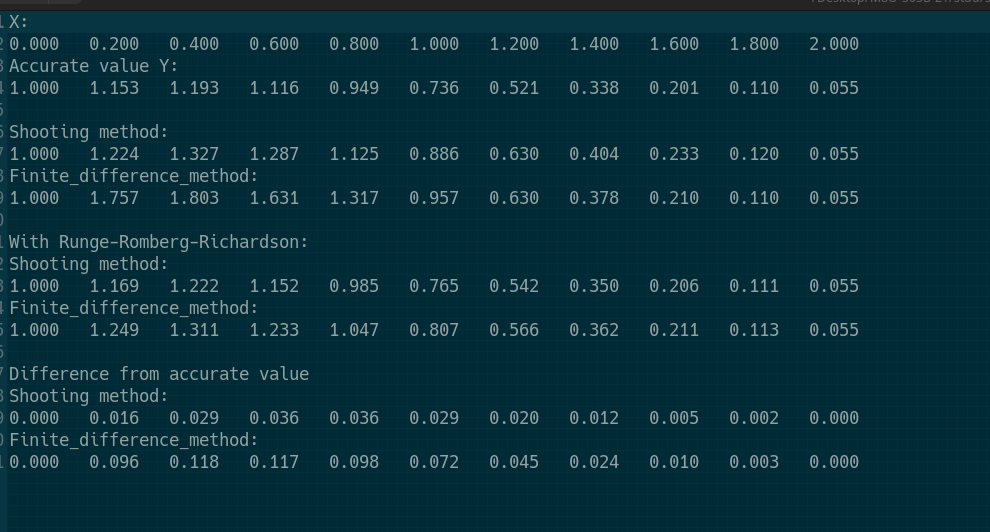
\includegraphics[width=.4\textwidth]{lab4.2}
\caption{Вывод в консоли}
\end{figure}


\subsection{Исходный код}
\lstinputlisting[title=\texttt{4-2.cpp}]{../stud/svoevolin/4-2.cpp}
\pagebreak